\documentclass[11pt]{article}
\usepackage[margin=1in]{geometry}
\usepackage{amsmath,amssymb,booktabs,graphicx,microtype}
\usepackage[numbers,sort&compress]{natbib}
\usepackage[hidelinks]{hyperref}
\graphicspath{{../results/figures/}}
\newcommand{\angstrom}{\ensuremath{\text{\normalfont\AA}}}
\renewcommand{\thesection}{S\arabic{section}}
\renewcommand{\thefigure}{S\arabic{figure}}
\renewcommand{\thetable}{S\arabic{table}}
\title{Supporting Information\\Common Spatial Witnesses Reveal Higher-Order Geometry in Molecular Path Barcodes}
\author{}
\date{}
\begin{document}
\maketitle

\section{Witness certificates and coordinate stability}

For a fixed selection, let $t^*$ and $x^*$ be a candidate optimum for the weighted one-center problem. Feasibility requires $\|x^*-x_v\|\leq r_v+t^*$ for every selected endpoint $v$. At $t^*>0$, let $I$ be a set of active endpoints for which equality holds. Optimality follows if zero is in the convex hull of their radial unit vectors $(x^*-x_v)/\|x^*-x_v\|$: this is the subgradient condition for minimizing the maximum of the endpoint clearances. At most four such vectors are needed in three dimensions. A feasible point at $t^*=0$ is already optimal because the scale is nonnegative. This condition is checked to numerical tolerance. In a union-valued family the global calculation also requires the minimum over selections, including valid lower bounds for skipped branches.

Suppose each endpoint moves by at most $\varepsilon$, with radii and patch memberships unchanged. At any trial point every endpoint clearance changes by at most $\varepsilon$ by the reverse triangle inequality. Taking the maximum of clearances, the nonnegative part, the minimum over points, and then the minimum over selections each preserves this uniform bound. Thus $|\tau'-\tau|\leq\varepsilon$. Taking the maximum over pairs gives the same bound on the pairwise birth. On a fixed graph this yields an additive interleaving for either rule under coordinate perturbation, by the same filtration-inclusion argument as in the main text. This statement holds on a fixed set of contacts.

\section{Event-based path persistence}

In each structure we fix the patch graph before comparing birth rules. We remove short-distance intramolecular clashes during RNA contact extraction (distance-to-sum-of-radii ratio $0.6$), not through an intermolecular protein--DNA clash prior. Each directed path uses its distinct patch set for support lookup, so paths with the same patch set share a support value even when the paths enter the chain complex in different orders. The symmetrized graph admits both orientations of each interaction adjacency; the birth rule is unchanged.

Both complexes are filtered on the ordered union of all finite birth values from the two rules. We form the allowed-boundary chain spaces and reduce the filtered boundary maps over a finite prime field; we report interval endpoints in \angstrom, not in units of event index. Missing or uncertified support is not assigned a zero value. The comparison of barcode multisets, the finite lifetime sum, and the plotted count are separate outputs. Interval counts throughout use a minimum length of $0.01\,\angstrom$ (bars strictly longer than this value); finite total persistence uses finite lifetimes and excludes essential intervals.

\begin{figure}[htbp]
\centering
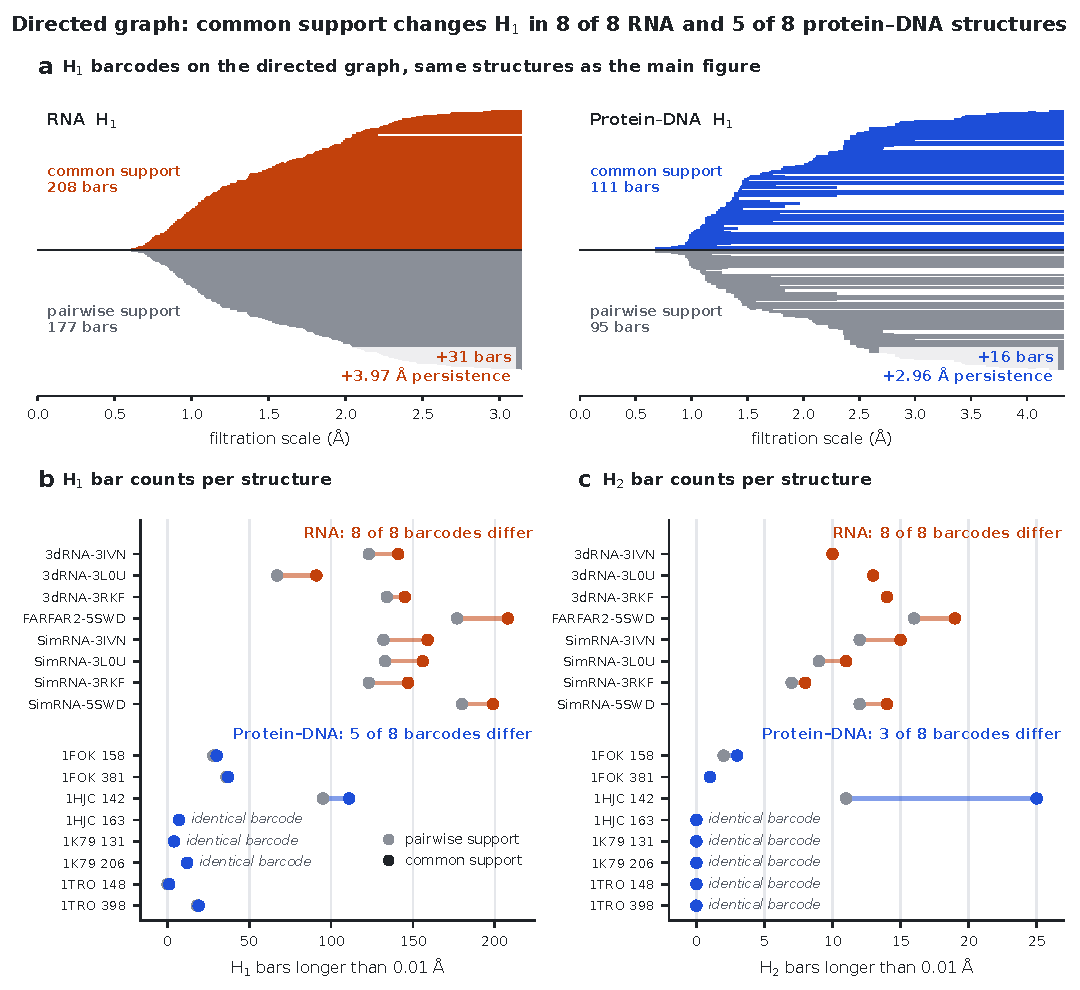
\includegraphics[width=\textwidth]{fig_common_support_directed.pdf}
\caption{\textbf{Common support changes higher-order barcodes even when the graph stays directed.}
Example $H_1$ intervals and structure-level counts for the directed graph are shown for both birth rules. The minimum bar length is $0.01\,\angstrom$. Intervals with right-edge arrows are essential. The interval multisets differ in both $H_1$ and $H_2$ for eight of eight RNA structures; for protein--DNA the counts of affected structures are five of eight in $H_1$ and three of eight in $H_2$. These counts of structures compare the interval multisets, not just the displayed numbers of bars.}
\label{fig:directed}
\end{figure}

\section{Nearest-witness coverage and steric filtering}

The input to the candidate generator is the macromolecular structure with the zinc and water coordinates withheld. A ligand group can offer multiple atoms, each with its own coordination ball. We enumerate pairwise-passing groups of ligands or polar groups, then evaluate the joint support for each candidate. Candidate witnesses are the solutions within the joint coordination tolerance. The independent steric check rejects witness points near nonligand heavy atoms; it does not change the solved witness. A hard negative in the candidate-composition audit is jointly infeasible at the tolerance, regardless of whether its optimal point at a larger scale is sterically admissible. Thus the filtered proportion uses a different denominator.

Nearest-witness coverage at radius $R$ counts each annotated site for which a candidate lies within $R$. One candidate can cover multiple annotations, and extra unmatched candidates do not decrease this coverage. The error summary is the median nearest-witness distance over annotated sites.

\paragraph{Time-separated zinc reference selection.}
The structure screen uses X-ray data, resolution and crystallographic free $R$ factor. The automated site screen checks zinc occupancy and displacement relative to surrounding ligands, macromolecular coordination and modeled ligand completeness. It excludes sites with symmetry-copy coordination or a recognized geometry-determining cofactor. These are coordinate-based checks; a release-date split makes no claim about sequence homology to the external models' training data. The external runs used Python 3.12 rather than the 3.10 specified in the run protocol; the pinned model code and released weights were unchanged.

\paragraph{All zinc annotations in the time-separated pool.}
We also evaluate the same predictions against all 86 zinc annotations from the same 32 structures, including sites that did not pass the automated checks. In this broader set, Metal3D covers a larger share of annotations at both radii; the joint geometry rule still gives the smallest median nearest-position error. These metrics distinguish coverage across all annotations from the proximity of candidate positions. Neither reports one-to-one detection precision or $F_1$.

\begin{table}[htbp]
\centering
\caption{\textbf{Across all zinc annotations, coverage and localization error favor different methods.} The three methods use the same 86 reference sites. Error is the median nearest-prediction distance over the reference set.}
\label{tab:all-zn}
\begin{tabular}{@{}lrrr@{}}
\toprule
Method & $1\,\angstrom$ coverage & $2\,\angstrom$ coverage & Median error (\angstrom) \\
\midrule
CS-PPH & 0.779 & 0.837 & 0.112 \\
Metal3D & 0.860 & 0.895 & 0.254 \\
AllMetal3D & 0.744 & 0.756 & 0.455 \\
\bottomrule
\end{tabular}
\end{table}

\section{Barcodes add discrimination on frozen hard pairs}

In FTDMP bound protein--DNA docking\citep{ftdmpdata}, we use target-grouped out-of-fold predictions against interface contact-area difference (CAD) scores. The first feature tier contains physical and pairwise-support summaries. The second adds higher-order support and support-difference summaries. The third adds barcode and persistence summaries. These are nested feature ablations of the same ranking setup, not external baselines.

Within each target and split, a hard pair combines a large absolute CAD-score difference with a small difference in the physical-plus-pairwise model's out-of-fold scores, using frozen within-target quantile rules. All tiers are evaluated on the exact same selected pairs for that target and split. A pair wins when the sign of the predicted ordering agrees with the sign of the CAD ordering. The pooled analysis averages split-level results within a target before resampling targets. The primary contrasts use paired target bootstrap intervals and target-level sign flips; the significance test for the barcode increment is Holm-adjusted.

\begin{table}[htbp]
\centering
\caption{\textbf{The barcode tier adds information on frozen protein--DNA hard pairs.} The benchmark contains 47 FTDMP bound targets; results pool the ten frozen split seeds. Differences and interval endpoints are in absolute win-rate units.}
\label{tab:hard}
\begin{tabular}{@{}lrrl@{}}
\toprule
Added features & Win-rate difference & Paired 95\% interval & $p$ \\
\midrule
Higher-order support summaries & $+0.0006$ & $[-0.0054,\,0.0064]$ & $0.84$ \\
Barcode and persistence summaries & $+0.0269$ & $[0.0129,\,0.0399]$ & $0.0006$ (Holm) \\
\bottomrule
\end{tabular}
\end{table}

On these fixed pairs, barcode features improve the ordering beyond what the same ranking setup obtains from support summaries. Pair selection uses the first tier, so gains in the third tier cannot change which pairs are evaluated.

\section{Same-pool external scoring context}

We report target-macro-average Spearman correlations on shared candidate pools. Published external scoring methods use their released implementations without fine-tuning on these test pools; our learned readout uses target-grouped out-of-fold predictions. The FTDMP official consensus combines scoring functions and is listed separately as a benchmark reference, not as a single-function baseline. These comparisons address global candidate ordering, not joint spatial feasibility.

\begin{table}[htbp]
\centering
\caption{\textbf{On the same PM pool, the CS-PPH readout ranks RNA decoys within the range of dedicated statistical potentials.} The pool contains 806 decoys from 20 targets, excluding native structures. Scores for our readout average 20 splits. The paired difference discussed below is computed separately on a single split.}
\label{tab:rna}
\begin{tabular}{@{}llr@{}}
\toprule
Scoring method & Role & Macro Spearman \\
\midrule
rsRNASP\citep{rsrnasp} & External statistical potential & 0.580 \\
cgRNASP\citep{cgrnasp} & External statistical potential & 0.560 \\
DFIRE-RNA\citep{dfirerna} & External statistical potential & 0.518 \\
CS-PPH feature readout & Target-grouped learned readout & 0.550 \\
lociPARSE\citep{lociparse} & External score; training overlap not verified & 0.596 \\
\bottomrule
\end{tabular}
\end{table}

On the single paired RNA split, the difference between our physical--topological--spectral readout and rsRNASP was $-0.032$ with interval $[-0.170,\,0.087]$; the interval contains zero, and the mean readout lies between DFIRE-RNA and cgRNASP. For lociPARSE, the overlap of the public weight training data with the PM targets was not verified, so its score supplies descriptive context, not an independent test.

\begin{table}[htbp]
\centering
\caption{\textbf{The CS-PPH readout outranks VoroMQA in both protein--DNA docking conditions.} Bound and unbound pools are evaluated separately. The CS-PPH readout is trained on target-grouped folds and reported out of fold; VoroMQA and the FTDMP consensus are used as released, without training on these pools. The FTDMP consensus combines several scoring functions and is an official reference ranking.}
\label{tab:pd}
\begin{tabular}{@{}lrr@{}}
\toprule
Scoring method & Bound macro Spearman & Unbound macro Spearman \\
\midrule
CS-PPH feature readout & 0.244 & 0.192 \\
VoroMQA\citep{voromqa} & $-0.004$ & $-0.032$ \\
FTDMP official consensus\citep{ftdmpdata} & 0.324 & $-0.011$ \\
\bottomrule
\end{tabular}
\end{table}

The bound pool contains 9{,}400 candidates over 47 targets. The paired bound difference from VoroMQA was $+0.248$ with interval $[0.194,\,0.305]$; from the FTDMP consensus it was $-0.079$ with interval $[-0.152,\,-0.005]$. VoroMQA spot checks reproduced 21 of 21 scores exactly. In the unbound condition, eight of 47 targets had any candidate with CAD score at least $0.3$. One 1BDT unbound candidate lacked a matching feature record and was excluded for every scoring method, leaving 18{,}799 candidates across both conditions in the shared comparison. Unbound correlations characterize ordering within that candidate-quality mix rather than the availability of near-native poses.

\bibliographystyle{unsrtnat}
\bibliography{refs}
\end{document}
